%%%%%%%%%%%%%%% LaTeX Compiler: XeLaTeX %%%%%%%%%%%%%%%

% License for LaTeX Configuration File

% This LaTeX configuration file is created by Lin, Xuanyu, HKUST, and is provided under the terms of the MIT License. You are free to use, copy, modify, merge, publish, distribute, sublicense, and/or sell copies of this configuration file, subject to the following conditions:

% 1. The above copyright notice and this license notice shall be included in all copies or substantial portions of the configuration file.

% 2. The configuration file is provided "as is", without warranty of any kind, express or implied, including but not limited to the warranties of merchantability, fitness for a particular purpose and noninfringement. In no event shall the authors or copyright holders be liable for any claim, damages or other liability, whether in an action of contract, tort or otherwise, arising from, out of or in connection with the configuration file or the use or other dealings in the configuration file.

% By using this configuration file, you agree to the terms and conditions of this license. If you do not agree to these terms and conditions, you must not use the configuration file.

\documentclass[10pt]{article}
% Text setting
% \usepackage{newtxtext}
\usepackage{setspace}
\usepackage[dvipsnames,svgnames]{xcolor}
\usepackage{comment}
% Chinese characters setup
\usepackage{fontspec}
\usepackage{xeCJK}
\setCJKmainfont{SimSun}
% Dealing with special characters
\usepackage[utf8]{inputenc}
% \usepackage[T1]{fontenc} % Conflict with fontspec & xeCJK
\usepackage{pifont}
% Mathematical formula typesetting
\usepackage{unicode-math}
\usepackage{amsmath}
\usepackage{amsfonts}
\usepackage{mathrsfs}
\setmathfont{Latin Modern Math}
% \usepackage{amssymb} % Contained in package unicode-math
% Jump (Math) \llbracket & \rrbracket
\usepackage{stmaryrd}
% Chemical formulas and equations
\usepackage[version=4]{mhchem}
% Graphics
\usepackage{graphicx}
\graphicspath{ {./images/} }
\usepackage[export]{adjustbox}
% Tables, enumeration
\usepackage{multirow}
\usepackage{caption}
\usepackage{subcaption}
\usepackage{enumitem}
% Adjust the position
\usepackage{float}
% Frames, reference
\usepackage{framed}
\usepackage[strict]{changepage}
\usepackage{hyperref}
\hypersetup{
	colorlinks=true,
	linkcolor=black,
	filecolor=magenta,      
	urlcolor=blue,
}
% Page & paragraph settings
\usepackage{fancyhdr}
\usepackage{geometry}
\geometry{left=1.5cm, right=1.5cm, top=2cm, bottom=2cm}
\usepackage{indentfirst}
\setlength{\parindent}{2em}
\setlength{\parskip}{0.5em}
% Algorithm & coding environment
\usepackage[ruled,vlined]{algorithm2e}
\usepackage[framemethod=TikZ]{mdframed}
\usepackage{listings}
\usepackage{wrapfig}
\usepackage{booktabs}
\usepackage{makecell}
% New command
\newcommand\course{PHYS 3031}  
\newcommand\coursetitle{Mathematical Methods in Physics II}
\newcommand\semester{Fall 2023}
\renewcommand{\labelenumi}{\alph{enumi}}
\newcommand{\Z}{\mathbb Z}
\newcommand{\R}{\mathbb R}
\newcommand{\Q}{\mathbb Q}
\newcommand{\NN}{\mathbb N}
\newcommand{\dd}{\mathrm{d}}
\DeclareMathOperator{\Mod}{Mod}
\renewcommand\lstlistingname{Algorithm}
\renewcommand\lstlistlistingname{Algorithms}
\def\lstlistingautorefname{Alg.}

%%%%%%%%%%%%%%% Page Setup %%%%%%%%%%%%%%%

\pagestyle{fancy}
\headheight 35pt
\lhead{\course\ \coursetitle\ \semester}
\rhead{
\includegraphics[width=2.5cm]{logo-hkust.png}}
\lfoot{}
\pagenumbering{arabic}
\cfoot{}
\rfoot{\small\thepage}
\headsep 1.2em

%%%%%%%%%%%%%%% Boxframe Setup %%%%%%%%%%%%%%%

\definecolor{blueshade}{rgb}{0.95,0.95,1} % Horizontal Line: DarkBlue
\definecolor{greenshade}{rgb}{0.90,0.99,0.91} % Horizontal Line: Green
\definecolor{redshade}{rgb}{1.00,0.90,0.90}% Horizontal Line: LightCoral
\definecolor{brownshade}{rgb}{0.99,0.97,0.93} % Horizontal Line: BurlyWood

\newenvironment{formal}[2]{%
	\def\FrameCommand{%
		\hspace{1pt}%
		{\color{#1}\vrule width 2pt}%
		{\color{#2}\vrule width 4pt}%
		\colorbox{#2}%
	}%
	\MakeFramed{\advance\hsize-\width\FrameRestore}%
	\noindent\hspace{-4.55pt}% Disable indenting first paragraph
	\begin{adjustwidth}{}{7pt}%
		\vspace{2pt}\vspace{2pt}%
	}
	{%
		\vspace{2pt}\end{adjustwidth}\endMakeFramed%
}

%%%%%%%%%%%%%%% Problem Environment Setup %%%%%%%%%%%%%%%

\mdfdefinestyle{problemstyle}{
	linecolor=black,linewidth=1pt,
	frametitlerule=true,
	frametitlebackgroundcolor=gray!20,
	roundcorner=10pt,
	innertopmargin=\topskip,
	frametitlealignment=\hspace{0em},
}

\mdfsetup{skipabove=\topskip,skipbelow=\topskip}
\mdtheorem[style=problemstyle]{Problem}{Problem}
\newenvironment{Solution}{\textbf{Solution.}}

%%%%%%%%%%%%%%% Coding Environment S6etup %%%%%%%%%%%%%%%

\lstset{
	basicstyle=\tt,
	% Line number
	numbers=left,
	rulesepcolor=\color{red!20!green!20!blue!20},
	escapeinside=``,
	xleftmargin=2em,xrightmargin=2em, aboveskip=1em,
	% Background frame
	framexleftmargin=1.5mm,
	frame=shadowbox,
	% Background color
	backgroundcolor=\color[RGB]{252,236,227},
	% Style
	keywordstyle=\color{blue}\bfseries,
	identifierstyle=\bf,
	numberstyle=\color[RGB]{0,192,192},
	commentstyle=\it\color[RGB]{0,153,51},
	stringstyle=\rmfamily\slshape\color[RGB]{128,0,0},
	% Show space
	showstringspaces=false
}

%%%%%%%%%%%%%%% Document Begins %%%%%%%%%%%%%%%

\begin{document}
	
%%%%%%%%%%%%%%% Title Page %%%%%%%%%%%%%%%

\begin{titlepage}
	\begin{center}
		\vspace*{3cm}
		
		\Huge
		\hrulefill
		\vspace{1cm}
		
		\huge
		\textbf{PHYS 3031 Course Notes\\}
		\vspace{1cm}
		\textbf{Mathematical Methods in Physics II}
		\vspace{1cm}
		
		\hrulefill
		
		\vspace{1.5cm}
		\Large

		\textbf{LIN, Xuanyu}
		
		\vfill
		
		$\mathscr{MATH\ METHODS\ IN\ PHYSICS}$
		
		\vspace{1cm}
		
		\course \ Mathematical Methods in Physics II
		
		\vspace{1cm}
		
		
\includegraphics[width=0.4\textwidth]{logo-hkust.png}
		\\
		
		\Large
		
		\today
		
	\end{center}
\end{titlepage}

%%%%%%%%%%%%%%% Article Begins %%%%%%%%%%%%%%%

\begin{comment}

\begin{abstract}
	Abstract Abstract Abstract Abstract Abstract Abstract Abstract Abstract Abstract Abstract Abstract Abstract Abstract Abstract Abstract Abstract Abstract Abstract Abstract Abstract Abstract Abstract Abstract Abstract Abstract Abstract Abstract Abstract Abstract Abstract Abstract Abstract Abstract
\end{abstract}

\tableofcontents

\begin{center}
	\section*{\LARGE Title}
\end{center}

\section{Section 1}

This is a link to \href{https://www.google.com}{Google}.

$$
\vec{\nabla} \cdot \vec{E}=\frac{1}{\epsilon_{0}} \cdot \rho
$$

\begin{formal}{DarkBlue}{blueshade}
	\textbf{Theorem 1.1} 这是一段中文。\hyperref[ref1]{[1]}
	
	$$
	\vec{\nabla} \cdot \vec{E}=\frac{1}{\epsilon_{0}} \cdot \rho
	$$
	
	\noindent This is an English sentence.
\end{formal}


\begin{center}
	\begin{tabular}{|c|c|c|}
		\hline
		\multirow{2}{*}{A} & B & C \\
		\cline{2-3}
		& D & E \\
		\hline
	\end{tabular}
\end{center}

\begin{algorithm}
	\SetAlgoLined
	\KwIn{$a, b$}
	\KwOut{$c$}
	$c = a + b$\;
	\Return{$c$}\;
	\caption{Addition}
\end{algorithm}

\begin{Problem}[Title]
	
	\lstset{language=Python}
	\begin{lstlisting}[tabsize=4]
print("Hello World!")
	\end{lstlisting}

\end{Problem}

\begin{Solution}
	
	Text
	
\end{Solution}

\newpage

\end{comment}

\tableofcontents

\newpage

\section{Series}

\subsection[Convergence Condition for Positive Series]{Convergence Condition for Positive Series $\sum\limits_{n=1}^{\infty} a_n$}

Necessary condition: $\lim_{N\to \infty} a_N = 0$

Hierarchy: $N! > a^N > N^b > \ln{N}$

\textbf{Stirling's Formula} $\ln{N!} \approx N\ln{N}-N \approx N\ln{N}$

\textbf{Comparison Test 1} $\sum a_n < \sum b_n$, $b$ converges $\to$ $a$ converges

\textbf{Comparison Test 2 (Integral Test)} $\sum a_n \& \int a(n) \dd n$ share the same fate

\textbf{Ratio Test}
	$\lim_{n\to \infty} \frac{a_{n+1}}{a_n} = \rho$, $\rho > 1 \to \text{Diverges}$, $\rho < 1 \to \text{Converges}$

\textbf{Extended (Special) Comparison Test}
$\lim_{n\to \infty} \frac{a_n}{b_n} = 1$, then $\sum a_n \& \sum b_n$ share the same fate

\subsection[Convergence Condition for Alternating Series]{Convergence Condition for Alternating Series $\sum\limits_{n=1}^{\infty} (-1)^n a_n$}

If $a_n>0, \lim_{n\to\infty} a_n = 0$, this series may diverge.

(1) Absolute Convergence: If $\sum a_n$ converges, then $\sum (-1)^n a_n$ converges

(2) Convergence Condition: $\lim_{n\to\infty} \text{ and } a_n > a_{n+1}$

(3) Diverge: If $a_n < a_{n+1}$, then the series diverges

\subsection[Power Series]{Power Series $\sum_{n=0}^\infty a_n (x-x_0)^n \rightarrow f(x)$}

Convergent condition for $x$:
$\lim_{n\to\infty} \big| \frac{a_{n+1}}{a_n} (x-x_0) \big| < 1$

\subsection{Asymptotic Series 渐近级数}

For functions $f(z)$ and $\phi(z)\neq 0$ defined in $\mathring{U}(z_0)$, we say that $f(z) = O(\phi(z))$ at $z\to z_0$ if $f(z)/\phi(z)$ is bounded, and that $f(z) = o(\phi(z))$ at $z\to z_0$ if $f(z)/\phi(z) \to 0$.

If for $\forall m$, when $z\to z_0$,
$$
f(z) - \sum_{n=0}^m a_n \phi_n(z) = o(\phi_m(z))
$$

we say that $\sum_{n=0}^m a_n \phi_n(z)$ is an asymptotic series for $f(z)$, even though the series may not converge:
$$
f(z) \sim \sum_{n=0}^m a_n \phi_n(z)
$$

\section[Taylor Expansion]{Taylor Expansion $\sum_{n=0}^\infty a_n (x-x_0)^n$}
$$
\sin x = \sum_{n=0}^\infty \frac{(-1)^n}{(2n+1)!} x^{2n+1}\ \ \ \ \ \cos x = \sum_{n=0}^\infty \frac{(-1)^n}{(2n)!} x^{2n}\ \ \ \ \ \tan x = x + \frac{x^3}{3} + \frac{2x^5}{15} + \frac{17x^7}{315} + ...\ \ \ \ \ e^{x} = \sum_{n=0}^\infty \frac{x^n}{n!}
$$

$$
\arctan x = \int_0^x \sum_{n=0}^\infty (-t^2)^n \dd t = \sum_{n=0}^\infty \frac{(-1)^n x^{2n+1}}{2n+1} \text{, where } |x| < 1
$$

\subsection{Leibniz Rule}
$$
\frac{\dd^{(M)}}{\dd x^M} (u\cdot v) = \bigg(\frac{\dd u}{\dd x}\frac{\partial}{\partial u} + \frac{\dd v}{\dd x}\frac{\partial}{\partial v}\bigg)^M (u\cdot v) = \sum_{n=0}^M C_M^n \bigg(\frac{\dd^{(M-n)} u}{\dd x^{(M-n)}}\bigg) \bigg(\frac{\dd^{(n)} v}{\dd x^n}\bigg)
$$

\subsection{Error Estimation when N Terms are Kept}
$$
f(x) \approx \sum_{n=0}^N (-1)^n a_n (x-x_0)^n\ \ \ \ \ b_n \equiv a_n(x-x_0)^n > 0
$$

\subsubsection[Alternating Series]{Alternating Series $S = \sum_{n=0}^\infty (-1)^n b_n$}

Maximum possible error for $f(x)$ is
$$
b_{N+1} = a_{N+1} \big| x-x_0 \big|^{N+1}
$$

\subsubsection["Positive" Series]{"Positive" Series $S = \sum_{n=0}^\infty a_n (x-x_0)^n, a_n (x-x_0)^n > 0$}

If it converges when $\big|x-x_0\big| < 1$, and $\big|a_{n+1}\big| < \big|a_n\big|$, then
$$
S - S_N < \frac{\big|a_{N+1}\big| \big|x-x_0\big|^{N+1}}{1-\big|x-x_0\big|}
$$

Note: In practice, Taylor Expansion is useful when $\big|x-x_0\big| << 1$, and an upper limit of error $\epsilon$ to be tolerated is given, even if the series converges for any value of $(x-x_0)$.

\subsection{L'Ĥopital's Rule}

Theorem 1:
$
\lim_{x\to x_0} \frac{f(x)}{g(x)} \overset{f(x_0)=0}{\underset{g(x_0)=0}\longrightarrow} \frac{0}{0}  \implies \lim_{x\to x_0} \frac{f(x)}{g(x)} \longrightarrow \frac{f'(x)}{g'(x)}
$

Theorem 2:
$
\lim_{x\to x_0} \frac{f(x)}{g(x)} \overset{f(x_0)=0}{\underset{g(x_0)=0}\longrightarrow} \frac{\infty}{\infty}  \implies \lim_{x\to x_0} \frac{f(x)}{g(x)} \longrightarrow \frac{f'(x)}{g'(x)} \text{(proved by the inverse of the fraction)}
$

\section{Complex Analysis}

Convergence of the Complex Series $\sum^\infty c_n = \sum^\infty a_n + i\sum^\infty b_n \implies a_n \text{and } b_n$ both converges.

Complex Power Series $\sum^\infty c_n z^n = f(z)$ with convergence region $\lim_{n\to\infty} \big|\frac{c_{n+1}}{c_n} z\big| < 1$.

Euler's Formula: $e^z = \cos z + i\sin z$ help solving the inverse trigonometric functions.

\subsection[Complex Functions]{Complex Functions $f(z) = f(x + iy) = u(x, y) + iv(x, y)$}

\textbf{Analytic Function}

Property: $f'(z) = \lim_{\Delta z \to 0} \frac{f(z+\Delta z) - f(z)}{\delta z}$ is \textbf{unique} regardless how $\Delta z \to 0$.

Necessary and Sufficient Conditions:

Cauchy-Riemann Conditions in Cartesian Coordinate: $\partial_x u = \partial_y v,\quad \partial_y u = -\partial_x v$

Cauchy-Riemann Conditions in Polar Coordinate: $\partial_\theta u = -\rho \partial_\rho v, \quad \partial_\theta v = \rho \partial_\rho u$

\textbf{Isolated Zeros 孤立零点}

If $f$ is analytic at $z_0$, then $f$ has a zeo of order $m\geq 1$ at $z_0$ if
$$
f(z_0) = f'(z_0) = \cdots = f^{(m-1)}(z_0) = 0
$$

and $f^{(m)}(z_0) \neq 0$. Note that $f$ becomes a \textbf{branch point} if $m$ is not an integer, and that $f$ is not analytic at that point.

\textbf{Theorem:} If $z=a$ is a zero of $f(z)$ which is not a constant at $\mathring{U}(a)$, then $\exists \rho > 0$, $f(z)$ doesn't have any zeros in the region $0 < |z-a| < \rho$.

\subsection{Line Integrals}

With the substitution of line $c: y = g(x)$, $\dd y = g'(x)\dd x$
$$
\lim_{\delta z_n\to 0} \sum_{z_n\in c} f(z_n) \Delta z_n = \int_c f(z)\dd z = \int_c f(x+iy)(\dd x + i\dd y) = \int_a^b f(x+ig(x))(1+ig'(x))\dd x \implies \int_c f(z)\dd z = -\int_{-c} f(z)\dd z
$$

\textbf{Cauchy's Theorem for Analytic Functions:}
$$
\oint_C f(z) \dd z = 0
$$

\textbf{Two Foundation Lemmas - Small \& Big Arc Lemma}

$\bullet$ Small Arc Lemma (小圆弧引理):

If $f(z)$ is continuous in $\mathring{U}(a)$, and $(z-a)f(z)$ approaches $k$ consistently as $|z-a|\to 0$ within $\theta_1 \leq \arg(z-a) \leq \theta_2$, then
$$
\lim_{\delta \to 0} \int_{C_{\delta}} f(z) \dd z = ik(\theta_2-\theta_1)
$$

$\bullet$ Big Arc Lemma (大圆弧引理):

If $f(z)$ is continuous in $\mathring{U}(\infty)$, and $zf(z)$ approaches $K$ consistently as $z \to \infty$ within $\theta_1 \leq \arg(z-a) \leq \theta_2$, then
$$
\lim_{R \to \infty} \int_{C_R} f(z) \dd z = iK(\theta_2-\theta_1)
$$

\textbf{Cauchy's Integral Formula:} $f(z)$ is analytic inside and on the contour, then for $\forall z_0$ inside the contour,
$$
\implies f(z_0) = \frac{1}{2\pi i} \oint_C \frac{f(z)\dd z}{z-z_0}\\
\implies f(z_0) = \frac{1}{2\pi} \int_0^{2\pi} f(z_0+Re^{i\theta}) \dd \theta \text{  (Mean Value Theorem 均值定理)}
$$

i.e. Get full information inside by the information on the boundary only.

\textbf{Note:} If $z_0$ were outside the contour, then

$\bullet$ If $f$ is analytic inside $C$, then $\frac{1}{2\pi i} \oint_C \frac{f(z)\dd z}{z-z_0} = 0$

$\bullet$ If $f$ is analytic outside $C$ and $\lim_{z\to\infty} f(z) = K$, then $\frac{1}{2\pi i} \oint_C \frac{f(z)\dd z}{z-z_0} = f(z_0) - K$

$\bullet$ The above two lemmas are NOT contradictory. In fact, if a complex function is analytic and bounded within $U(\infty)$, then it must be a constant function.

\textbf{Liouville Theorem (in Complex Analysis) 刘维尔定理}

Every bounded entire function must be constant. That is, every holomorphic function $f$ for which there exists a positive number $M$ such that $|f(z)|\leq M$ for all $z\in\mathbb{C}$ is constant. Equivalently, non-constant holomorphic functions on $\mathbb{C}$ have unbounded images.

\textbf{Poisson's Formula}

Idea: If $f(z=x+iy) = u(x, y) + iv(x, y)$ is analytic on the upper-half plane and that we only know the value of $u(x, 0)$ or $v(x, 0)$, we can first get the value of $f(x\in\R)$, then apply the Cauchy's Integral Formula to get all the complex value on the upper-half plane:
$$
f(z) = \frac{1}{\pi i} \int_{-\infty}^{\infty} \frac{u(\xi,0)}{\xi-(x+iy)} \dd \xi = \frac{1}{\pi} \int_{-\infty}^{\infty} \frac{v(\xi,0)}{\xi-(x+iy)} \dd \xi
$$
$$
f(z) = \frac{y}{\pi} \int_{-\infty}^{\infty} \frac{f(\xi)}{(\xi-x)^2+y^2} \dd \xi = \frac{1}{\pi i} \int_{-\infty}^{\infty} \frac{(\xi-x)f(\xi)}{(\xi-x)^2+y^2} \dd \xi
$$

\subsection{Taylor Series}

\textbf{Derivative of $f(z)$}
$$
f^{(n)}(a) \equiv \frac{\dd^{(n)}f}{\dd a^n} = \frac{n!}{2\pi i} \oint_C \frac{f(z) \dd z}{(z-a)^{n+1}}
$$
\begin{wrapfigure}{r}{0.14\textwidth}
	\centering
	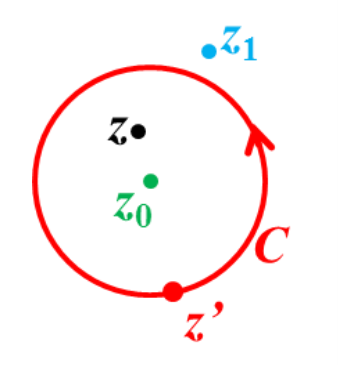
\includegraphics[width=0.14\textwidth]{img3-1}
\end{wrapfigure}

\textbf{Taylor Series $f(z) = \sum a_n (z-z_0)^n$}

Suppose $f(z)$ has a singular point at $z_1$, we can expand $f(z)$ at $z_0$:
$$
f(z) = \frac{1}{2\pi i} \oint_C \frac{f(z')\dd z'}{z'-z} = \frac{1}{2\pi i} \sum_{n=0}^{\infty} (z-z_0)^n \oint_C \frac{f(z')\dd z'}{(z'-z_0)^{n+1}} = \sum_{n=0}^{\infty} a_n (z-z_0)^n
$$
$$
a_n \equiv \frac{1}{2\pi i} \oint_C \frac{f(z')\dd z'}{(z'-z_0)^{n+1}} = \frac{1}{n!} \frac{\dd^n f(z_0)}{\dd z^n}
$$

\subsection{Lauren Series}

Suppose $f(z)$ has a pole at $z_0$, define the hole as order $N \geq 1$ at $z_0$ if $\lim_{z\to z_0} (z-z_0)^N f(z)$ is finite and non-zero. ("Essential Pole" if such $N\to\infty$ like $e^{1/z}$ at $z=0$)

$f(z)$ can be expressed as
$$
f(z) = \sum_{m=0}^\infty a_m (z-z_0)^m + \sum_{n=1}^N \frac{b_m}{(z-z_0)^n} \text{ as } \lim_{z\to z_0} (z-z_0)^N f(z) = b_N
$$
\begin{wrapfigure}{r}{0.14\textwidth}
	\centering
	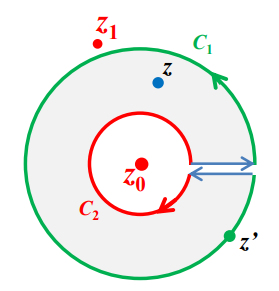
\includegraphics[width=0.14\textwidth]{img3-2}
\end{wrapfigure}
$$
f(z) = \frac{1}{2\pi i} \oint_{C_1} \frac{f(z')\dd z'}{z'-z} + \oint_{C_2} \frac{f(z')\dd z'}{z'-z} = I_1 + I_2
$$
We have
$$
a_n = \frac{1}{2\pi i} \oint_{C_1} \frac{f(z')\dd z'}{(z'-z_0)^{n+1}} \quad b_1 = \frac{1}{2\pi i} \oint_{C_2} f(z')\dd z' \quad b_{n+1} = \frac{1}{2\pi i} \oint_{C_2} f(z')(z'-z_0)^n\dd z' \quad \text{(Not Useful)}
$$
Note that when $f(z)$ is analytic at $z_0$, $a_n$ becomes the same as the coefficient in Taylor Series, and $b_i \equiv 0$ for $\forall i$.

\subsection{Analytic Continuation 解析延拓}

Suppose $f_1(z)$ is analytic in region $g_1$, $f_2(z)$ is analytic in region $g_2$, such that $g_1 \cap g_2 \neq \emptyset$. If $f_1(z) \equiv f_2(z)$ in $g_1 \cap g_2$, then $f_2(z)$ is the analytic continuation for $f_1(z)$ in region $g_2$.

\subsection{Residue Theorem 留数定理}
We want to evaluate $\oint_C f(z) \dd z$ around the pole. By applying the Lauren Series, one can prove that
$$
\oint_C f(z) \dd z = 2\pi i b_1
$$

\newpage

To find $b_1$, notice that $\lim_{z\to z_0} (z-z_0)^N f(z)$ is finite and all the other terms in the Lauren Series would disappear by taking $(N-1)$ times derivatives and taking $z = z_0$:
$$
b_1 = \lim_{z\to z_0} \frac{g^{(M-1)}(z)}{(M-1)!}, \text{ where } g(z) \equiv (z-z_0)^M f(z), M\geq N \text{ (Usually taking $M=N$)}
$$

We then define the coefficient $b_1$ of the Lauren Series at the pole $z_0$ as $b_1(z_0) \equiv R(z_0)$, and refer as the \textbf{residue} of $f(z)$ at $z_0$

\begin{figure}[h]
	\centering
	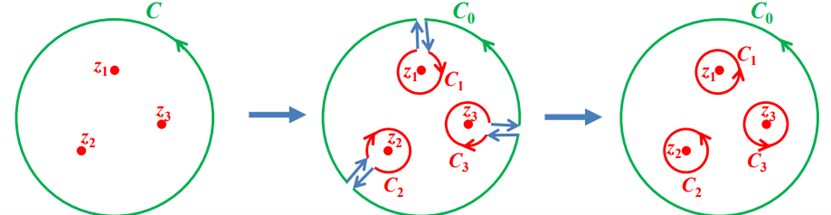
\includegraphics[width=0.5\textwidth]{img3-3}
\end{figure}

If $f(z)$ has singular points $z_1, z_2, \cdots, z_n$ inside contour $C$, then
$$
\oint_C f(z)\dd z = 2\pi i \sum_{n=1}^N R(z_n)
$$

\textbf{Residue at Infinity}

If $\infty$ is NOT a non-isolated singularity, define
$$
R(f(\infty)) = \frac{1}{2\pi i} \oint_{C'} f(z) \dd z
$$
where $C'$ is a closed curve \textbf{clockwise} around a point at infinity.

Note that
$$
\begin{aligned}
	R(f(\infty)) &= \frac{1}{2\pi i} \oint_{C'} f(z) \dd z = - \frac{1}{2\pi i} \oint_{C'} \frac{f(1/t)}{t^2} \dd t\\
	&= - \frac{f(1/t)}{t^2} \text{\quad$t^{-1}$'s coefficient expanding at $t=0$}\\
	&= - f(1/t) \text{\quad$t^{1}$'s coefficient expanding at $t=0$}\\
	&= - f(z) \text{\quad$z^{-1}$'s coefficient expanding at $z=\infty$}
\end{aligned}
$$
Note: $R(f(\infty))$ may NOT be zero even if $f(z)$ is analytic at $z=\infty$.



\newpage

\begin{table}[H]
	\centering
	\begin{tabular}{|c|c|}
		\hline
		Noun & Explanation \\
		\hline
		Analytic (Holomorphic) Point & A point which the function has a derivative at and in a neighborhood around that point \\
		
		Branch Point 分枝点& A point such that all of its neighborhoods contain a point that has more than n values \\
		
		Pole 极点& A point of a function $f$ if it is a zero of the function $1/f$ which is analytic \\
		
		Regular Point & A point in the function's domain where the function is differentiable \\
		
		Singularity 奇点& \thead{Essential Singularity 本性奇点: $\lim_{z\to z_0} (z-z_0)^N f(z)$ is always infinite \\ Isolated Singularity 孤立奇点: One that has no other singularities close to it \\ Movable Singularity, Removable Singularity } \\

		\hline
	\end{tabular}
\caption{Explanation of Important Nouns}
\end{table}
























\newpage

\end{document}

\begin{comment}

\section*{Homework 1}

\begin{Problem}
	
	Use the comparison test to prove the convergence of the following series:
	
	\noindent (a) $\sum_{n=1}^\infty \frac{1}{2^n+3^n}$
	
	\noindent (b) $\sum_{n=1}^\infty \frac{1}{n 2^n}$
	
\end{Problem}

\textbf{Solution.}

(a) By considering the n-th term, we have

$$
\frac{1}{2^n+3^n} < \frac{1}{2^n+2^n} = \frac{1}{2^{n+1}}
$$

Since the series is positive and that

$$
\sum_{n=1}^\infty \frac{1}{2^{n+1}} = \frac{1}{2} < \infty,
$$

the original series converges.

(b) Consider the n-th term, we have

$$
\frac{1}{n 2^n} < \frac{1}{2^n}
$$

for $n \geq 2$.

Since the series is positive and that

$$
\sum_{n=1}^\infty \frac{1}{n 2^n} < \frac{1}{2} + \sum_{n=2}^\infty \frac{1}{2^n} = 1 < \infty,
$$

the original sequence converges.

\newpage

\begin{Problem}
	
	Test the following series for convergence using the comparison test:
	
	\noindent (a) $\sum_{n=1}^\infty \frac{1}{\sqrt{n}}$
	
	\noindent (b) $\sum_{n=2}^\infty \frac{1}{\ln{n}}$
	
\end{Problem}

\textbf{Solution.}

(a) Consider the n-th term, we have

$$
\frac{1}{\sqrt{n}} > \frac{1}{n}
$$

for $n \geq 2$.

Since

$$
\sum_{n=1}^\infty \frac{1}{\sqrt{n}} > 1 + \sum_{n=2}^\infty \frac{1}{n} \to \infty,
$$

the series diverges by the comparison test.

(b) Since $\ln n < n$ for $\forall n \in \NN$,

$$
\sum_{n=2}^\infty \frac{1}{\ln{n}} > \sum_{n=2}^\infty \frac{1}{n} \to \infty
$$

Thus, the series diverges by the comparison test.

\newpage

\begin{Problem}
	
	Use the integral test to find whether the following series converge or diverge:
	
	\noindent (a) $\sum_{n=2}^\infty \frac{1}{n\ln{n}}$
	
	\noindent (b) $\sum_{n=1}^\infty \frac{e^n}{e^{2n}+9}$
	
\end{Problem}

\textbf{Solution.}

(a) Consider the integral

$$
\int_2^\infty \frac{1}{x \ln x} \dd x = \int_{\ln 2}^\infty \frac{\dd \ln x}{\ln x} = \ln \ln x \big|_2^\infty \to \infty
$$

Thus, the original series diverges.

(b) Consider the integral

$$
\int_2^\infty \frac{e^x}{e^{2x}+9} \dd x = \int_2^\infty \frac{1}{e^x+\frac{9}{e^x}} \dd x \geq \int_2^\infty \frac{1}{2e^x} = -\frac{1}{2} e^{-x} \big|_2^\infty = \frac{e^{-2}}{2} < \infty
$$

Thus, the original series converges.

\newpage

\begin{Problem}
	
	Use the ratio test to find whether the following series converge or diverge:
	$\sum_{n=0}^\infty \frac{(n!)^3 e^{3n}}{(3n)!}$
	
\end{Problem}

\textbf{Solution.}

The n-th term is given by

$$
a_n = \frac{(n!)^3 e^{3n}}{(3n)!}
$$

Thus,

$$
\frac{a_{n+1}}{a_n} = \frac{[(n+1)!]^3 e^{3(n+1)}}{[3(n+1)]!} \frac{(3n)!}{(n!)^3 e^{3n}} = \frac{(n+1)^3 \cdot e^3}{(3n+1)(3n+2)(3n+3)} = e^3 \cdot \frac{n^3+3n^2+3n+1}{27n^3+54n^2+33n+6}
$$

$$
\lim_{n\to \infty} \frac{a_{n+1}}{a_n} = \lim_{n\to \infty} e^3 \cdot \frac{n^3+3n^2+3n+1}{27n^3+54n^2+33n+6} = \lim_{n\to \infty} e^3 \cdot \frac{1+\frac{3}{n}+\frac{3}{n^2}+\frac{1}{n^3}}{27+\frac{54}{n}+\frac{33}{n^2}+\frac{6}{n^3}} = \frac{e^3}{27} < 1
$$

Thus, the series converges by the ratio test.

\newpage

\begin{Problem}
	
	Use the special comparison test to find whether the following series converge or diverge:
	
	\noindent (a) $\sum_{n=9}^\infty \frac{(2n+1)(3n-5)}{\sqrt{n^2-73}}$
	
	\noindent (b) $\sum_{n=3}^\infty \frac{(n-\ln{n})^2}{5n^4-3n^2+1}$
	
	\noindent (c) $\sum_{n=1}^\infty \frac{\sqrt{n^3+5n-1}}{n^2-\sin n^3}$
	
\end{Problem}

\textbf{Solution.}

(a)

$$
a_n = \frac{(2n+1)(3n-5)}{\sqrt{n^2-73}}
$$

Consider another sequence with $b_n = 6n$. Obviously, $\sum b_n$ diverges.

$$
\lim_{n \to \infty} \frac{a_n}{b_n} = \lim_{n \to \infty} \frac{(2n+1)(3n-5)}{6n \sqrt{n^2-73}} = \lim_{n \to \infty} \frac{6-\frac{7}{n}-\frac{5}{n^2}}{6 \sqrt{1-\frac{73}{n^2}}} = 1
$$

Thus, $\sum a_n$ also diverges.

(b)

$$
a_n = \frac{(n-\ln{n})^2}{5n^4-3n^2+1}
$$

Consider another sequence with $b_n = \frac{1}{5n^2}$. Obviously, $\sum b_n$ converges.

$$
\lim_{n \to \infty} \frac{a_n}{b_n} = \lim_{n \to \infty} \frac{5n^2 (n-\ln{n})^2}{5n^4-3n^2+1} = \lim_{n \to \infty} \frac{(1-\frac{\ln n}{n})^2}{1-\frac{3}{5n^2}+\frac{1}{5n^4}} = 1
$$

Thus, $\sum a_n$ also converges.

(c)

$$
a_n = \frac{\sqrt{n^3+5n-1}}{n^2-\sin n^3}
$$

Consider another sequence with $b_n = \frac{1}{n^{\frac{1}{2}}}$. Then $\sum b_n$ diverges from the previous problem.

$$
\lim_{n \to \infty} \frac{a_n}{b_n} = \lim_{n \to \infty} \frac{\sqrt{n^4+5n^2-n}}{n^2-\sin n^3} = \lim_{n \to \infty} \frac{\sqrt{1+\frac{5}{n^2}-\frac{1}{n^3}}}{1-\frac{\sin n^3}{n^2}} = 1
$$

as

$$
0 = \lim_{n \to \infty} -\frac{1}{n^2} \leq \lim_{n \to \infty} \frac{\sin n^3}{n^2} \leq \lim_{n \to \infty} \frac{1}{n^2} = 0
$$

Thus, $\sum a_n$ also diverges.

\newpage

\begin{Problem}
	
	Test the following series for convergence:
	
	\noindent (a) $\sum_{n=1}^\infty \frac{(-1)^n}{\sqrt{n}}$
	
	\noindent (b) $\sum_{n=1}^\infty \frac{(-2)^n}{n^2}$
	
\end{Problem}

\textbf{Solution.}

(a) Since

$$
\frac{|a_{n+1}|}{|a_n|} = \frac{\sqrt{n}}{\sqrt{n+1}} < 1
$$

and

$$
\lim_{n \to \infty} a_n = \lim_{n \to \infty} \frac{(-1)^n}{\sqrt{n}} = 0
$$

Thus, the original series converges.

(b)

$$
\lim_{n \to \infty} \frac{a_{n+1}}{a_n} = \lim_{n \to \infty} -\frac{2n^2}{(n+1)^2} = \lim_{n \to \infty} -\frac{2}{(\frac{n+1}{n})^2} = -2
$$

Thus, the original series diverges.

\newpage

\section*{Homework 2}

\begin{Problem}
	
	Find the interval of convergence of the following power series; be sure to investigate the endpoints of the interval: $\sum_{n=1}^\infty \frac{(-1)^n (x+1)^n}{n}$
	
\end{Problem}

\textbf{Solution.}

$$
a_n = \frac{(-1)^n (x+1)^n}{n} \implies \rho_n = \big| \frac{a_{n+1}}{a_n} \big| = \big| \frac{(-1)^{n+1} (x+1)^{n+1}}{n+1} \frac{n}{(-1)^n (x+1)^n} \big| = \frac{n}{n+1}\big|x+1\big|
$$

Thus,

$$
\rho = \lim_{n\to\infty} \rho_n = \big|x+1\big|
$$

For the interval of convergence, we have

$$
\rho < 1 \implies \big|x+1\big| < 1 \implies x \in (-2, 0)
$$

When $x = -2$,

$$
\sum_{n=1}^\infty \frac{(-1)^n (x+1)^n}{n} = \sum_{n=1}^\infty \frac{1}{n} \text{  Diverges}
$$

When $x = 0$,

$$
\sum_{n=1}^\infty \frac{(-1)^n (x+1)^n}{n} = \sum_{n=1}^\infty \frac{(-1)^n}{n} \text{  Converges}
$$

Thus, the interval of convergence is $\left(-2,0\right]$.

\newpage

\begin{Problem}
	
	The following series are not power series, but you can transform each one into a power
	series by a change of variable and so find out where it converges:
	
	\noindent (a) $\sum_{n=2}^\infty \frac{(-1)^n x^{n/2}}{n \ln n}$
	
	\noindent (b) $\sum_{n=0}^\infty (\sqrt{x^2+1})^n \frac{2^n}{3^n+n^3}$
	
	\noindent (c) $\sum_{n=0}^\infty (\sin x)^n (-1)^n 2^n$
	
\end{Problem}

\textbf{Solution.}

(a) Let $y = x^{1/2}$, then $a_n = \frac{(-1)^n y^n}{n \ln n}$

$$
\rho = \lim_{n\to\infty} \big| \frac{a_{n+1}}{a_n} \big| = \lim_{n\to\infty} \big| \frac{(-1)^{n+1} y^{n+1}}{(n+1) \ln (n+1)} \frac{n \ln n}{(-1)^n y^n} \big| = \lim_{n\to\infty} \frac{n \ln n}{(n+1) \ln (n+1)} \big| y \big| = \lim_{n\to\infty} \frac{\ln n + 1}{\ln (n+1) + 1} \big| y \big| = \big| y \big|
$$

For the interval of convergence, we have

$$
\rho < 1 \implies \big|y\big| < 1 \implies y \in (-1, 1) \implies x \in \left[0, 1\right)
$$

When $x = 1$,

$$
\sum_{n=2}^\infty \frac{(-1)^n x^{n/2}}{n \ln n} = \sum_{n=2}^\infty \frac{(-1)^n}{n \ln n}
$$

It converges since it's an alternating series with $\big| a_n \big| > \big| a_{n+1} \big|$.

Thus, the interval of convergence is $[0,1]$.

(b) Let $y = \sqrt{x^2+1}$, then $a_n = y^n \frac{2^n}{3^n+n^3}$

$$
\rho = \lim_{n\to\infty} \big| \frac{a_{n+1}}{a_n} \big| = \lim_{n\to\infty} \big| \frac{y^{n+1}}{y^n} \frac{2^{n+1}}{3^{n+1}+(n+1)^3} \frac{3^n+n^3}{2^n} \big| = \lim_{n\to\infty} \big| 2y \frac{1+\frac{n^3}{3^n}}{3+\frac{(n+1)^3}{3^n}} \big| = \frac{2}{3} y
$$

For the interval of convergence, we have

$$
\rho < 1 \implies \big|\frac{2}{3} y\big| < 1 \implies y \in (-\frac{3}{2}, \frac{3}{2}) \implies x \in \left[0, \frac{\sqrt{5}}{2}\right)
$$

When $x = \frac{\sqrt{5}}{2}$,

$$
\sum_{n=0}^\infty (\sqrt{x^2+1})^n \frac{2^n}{3^n+n^3} = \sum_{n=0}^\infty (\frac{3}{2})^n \frac{2^n}{3^n+n^3} = \sum_{n=0}^\infty \frac{1}{1+\frac{n^3}{3^n}} > \sum_{n=0}^\infty \frac{1}{1+n} \text{Diverges}
$$

(c) Let $y = \sin x$, then $a_n = (-2y)^n$

$$
\rho = \lim_{n\to\infty} \big| \frac{a_{n+1}}{a_n} \big| = 2 \big| y \big|
$$

For the interval of convergence, we have

$$
\rho < 1 \implies y \in (-\frac{1}{2}, \frac{1}{2}) \implies x \in \left(-\frac{\pi}{6} + k\pi, \frac{\pi}{6} + k\pi\right)
$$

When $x = -\frac{\pi}{6} + k\pi$ or $\frac{\pi}{6} + k\pi$, the series doesn't converge.

\newpage

\begin{Problem}
	
	Find the first few terms of the Maclaurin series for the following functions and check your results by computer: $\frac{e^x}{1-x}$
	
\end{Problem}

\textbf{Solution.}

$$
e^x = 1 + x + \frac{x^2}{2!} + \frac{x^3}{3!} + \dots
$$

$$
\frac{1}{1-x} = 1 + x + x^2 + x^3 + \dots
$$

$$
\implies \frac{e^x}{1-x} = 1 + 2x + \frac{5}{2}x^2 + \frac{8}{3}x^3 + \dots
$$

\newpage

\begin{Problem}
	
	Show that $\ln (1−x) = −x$ with an error less than 0.0056 for $|x| < 0.1$.
	
\end{Problem}

\textbf{Solution.}

According to Taylor Series,

$$
\ln (1−x) = -x - \frac{x^2}{2} - \frac{x^3}{3} - \frac{x^4}{4} - \dots
$$

$$
\implies \big| \ln(1-x) - (-x) \big| \leq \frac{|x|^2}{2} + \frac{|x|^3}{3} + \frac{|x|^4}{4} + \dots \leq \frac{0.1^2}{2} + \frac{0.1^3}{3} + \frac{0.1^4}{4} + \dots \leq 0.005 + 0.0004 + 0.000111... < 0.0056
$$

\newpage

\begin{Problem}
	
	Show that $2/\sqrt{4-x} = 1+\frac{1}{8}x$ with an error less than $\frac{1}{32}$ for $0<x<1$.
	
\end{Problem}

\textbf{Solution.}

According to the Taylor Series,

$$
\frac{2}{\sqrt{4-x}} = 1 + \frac{x}{8} + \frac{3x^2}{128} + \frac{5x^3}{1024} + \cdots
$$

Error:

$$
S - S_N < \frac{\big|a_{N+1}\big| \big|x-x_0\big|^{N+1}}{1-\big|x-x_0\big|} = \frac{\big|a_2\big| \big|x\big|^2}{1-\big|x\big|} = \frac{3x^2}{128(1-x)} < \frac{3}{128} < \frac{1}{32}
$$


\newpage

\begin{Problem}
	
	Use power series to evaluate the function at the given point. Compare with computer results, using the computer to find the series, and also to do the problem without series. Resolve any disagreement in results: $e^{\arcsin{x}} + \ln (\frac{1-x}{e})$ at $x = 0.0003$
	
\end{Problem}

\textbf{Solution.}

According to Taylor Series at $x=0$,

$$
\begin{aligned}
	e^{\arcsin{x}} + \ln (\frac{1-x}{e}) &\approx e^{x+\frac{x^3}{6}} - (1 + x + \frac{x^2}{2} + \frac{x^3}{3} + \frac{x^4}{4} + \cdots)\\
	&\approx [1 + x + \frac{x^3}{6} + \frac{1}{2} (x + \frac{x^3}{6})^2 + \frac{1}{6} (x + \frac{x^3}{6})^3 + \cdots] - [1 + x + \frac{x^2}{2} + \frac{x^3}{3} + \frac{x^4}{4} + \cdots]\\
	&\approx [1 + x + \frac{1}{2} x^2 + \frac{1}{3} x^3 + \frac{5}{24} x^4] - [1 + x + \frac{x^2}{2} + \frac{x^3}{3} + \frac{x^4}{4}]\\
	&= -\frac{1}{24} x^4 = -\frac{1}{24} (3\times 10^{-4})^4 \approx 3\times 10^{-16}
\end{aligned}
$$

\newpage

\begin{Problem}
	
	Use Maclaurin series to evaluate each of the following. Although you could do them by
	computer, you can probably do them in your head faster than you can type them into the
	computer. So use these to practice quick and skillful use of basic series to make simple
	calculations: $\frac{\dd^3}{\dd x^3} (\frac{x^2 e^x}{1-x})$ at $x = 0$
	
\end{Problem}

\textbf{Solution.}

$$
\frac{x^2 e^x}{1-x} = x^2 \cdot (1 + x + \frac{x^2}{2} + \frac{x^3}{6} + \dots) \cdot (1 + x + x^2 + x^3 + \dots) = x^2 + 2x^3 + \frac{5}{2} x^4 + \cdots
$$

Thus,

$$
\frac{\dd^3}{\dd x^3} (\frac{x^2 e^x}{1-x}) \bigg|_{x=0} = \frac{\dd^3}{\dd x^3} (x^2 + 2x^3 + \frac{5}{2} x^4 + \cdots) \bigg|_{x=0} = 12
$$

\newpage

\begin{Problem}
	
	Find the sum of the following series by recognizing it as the Maclaurin series for a function evaluated at a point: $\sum_{n=1}^\infty \frac{1}{n 2^n}$
	
\end{Problem}

\textbf{Solution.}

Maclaurin series:

$$
f(x) = \sum_{n=0}^\infty \frac{f^{(n)}(0)}{n!} x^n
$$

Consider the function:

$$
f(x) = \log (1+x) = \sum_{n=1}^\infty \frac{(-1)^{n-1}}{n} x^n
$$

When $x = -\frac{1}{2}$, we have

$$
\sum_{n=1}^\infty \frac{(-1)^{n-1}}{n} (-\frac{1}{2})^n = -\sum_{n=1}^\infty \frac{1}{n 2^n} = \log(1-\frac{1}{2}) = -\log 2
$$

$$
\implies \sum_{n=1}^\infty \frac{1}{n 2^n} = \log 2
$$

\newpage

\begin{Problem}
	
	Evaluate the following indeterminate forms by using L'Hopital's rule and check your
	results by computer. (Note that Maclaurin series would not be useful here because
	x does not tend to zero, or because a function (ln x, for example) is not expandable in a Maclaurin series.): $\lim_{x \to \pi} \frac{x \sin x}{x-\pi}$
	
\end{Problem}

\textbf{Solution.}

By L'Hopital's Rule,

$$
\lim_{x \to \pi} \frac{x \sin x}{x-\pi} = \frac{\sin x + x \cos x}{1} \bigg|_{x=\pi} = -\pi
$$

\newpage

\section*{Homework 3}

\begin{Problem}
	
	Test each of the following series for convergence:
	
	\noindent (a) $\sum e^{in\pi/6}$
	
	\noindent (b) $\sum \frac{i^n}{n}$
	
	\noindent (c) $\sum \big(\frac{1+i}{1-i\sqrt{3}}\big)^n$
	
\end{Problem}

\textbf{Solution.}

(a)

$$
\sum e^{in\pi/6} = \lim_{n\to\infty} \frac{e^{i(n+1)\pi/6} - e^{i\pi/6}}{e^{i\pi/6} - 1} = \frac{\lim_{n\to\infty} e^{i(n+1)\pi/6} - e^{i\pi/6}}{e^{i\pi/6} - 1} \text{ Doesn't converge.}
$$

(b)

$$
\lim_{n\to\infty} \big|\frac{a_{n+1}}{a_n}\big| = \lim_{n\to\infty} \big|\frac{n}{n+1} i\big| = 1
$$

$$
\sum \frac{i^n}{n} = \sum_{n=0}^\infty \bigg(-\frac{1}{4n+2}+\frac{1}{4n+4}\bigg) + \bigg(\frac{1}{4n+1}-\frac{1}{4n+3}\bigg) i
$$

Note that both series converges as they meet the condition for the convergence for altenating series. Thus, the series converges.

(c)

$$
\sum \bigg(\frac{1+i}{1-i\sqrt{3}}\bigg)^n = \sum \bigg(\frac{\sqrt{2} e^{i\pi/4}}{2 e^{-\pi/6}}\bigg)^n
$$

$$
\lim_{n\to\infty} \big|\frac{a_{n+1}}{a_n}\big| = \lim_{n\to\infty} \big|\frac{\sqrt{2}}{2}\big| < 1
$$

Thus, the series converges.

\newpage

\begin{Problem}
	
	Find the disk of convergence for each of the following complex power series:
	
	\noindent (a) $\sum_{n=1}^{\infty} \frac{z^{2n}}{(2n+1)!}$
	
	\noindent (b) $\sum_{n=1}^{\infty} \frac{z^n}{\sqrt{n}}$
	
	\noindent (c) $\sum_{n=1}^{\infty} \frac{(iz)^n}{n^2}$
	
	\noindent (d) $\sum_{n=0}^{\infty} \frac{(z-2+i)^n}{2^n}$
	
\end{Problem}

\textbf{Solution.}

(a)
$$
\lim_{n\to\infty} \big|\frac{a_{n+1}}{a_n}\big| = \lim_{n\to\infty} \big|\frac{z^2}{(2n+2)(2n+3)}\big| = 0 < 1 \text{ for } \forall z
$$

Thus, it converges for any $z$.

(b)
$$
\lim_{n\to\infty} \big|\frac{a_{n+1}}{a_n}\big| = \lim_{n\to\infty} \big|\frac{\sqrt{n}}{\sqrt{n+1}} z\big| = \big|z\big| < 1
$$

Thus, it converges for $\big|z\big| < 1$.

(c)
$$
\lim_{n\to\infty} \big|\frac{a_{n+1}}{a_n}\big| = \lim_{n\to\infty} \big|\frac{\sqrt{n^2}}{\sqrt{(n+1)^2}} iz\big| = \big|z\big| < 1
$$

Thus, it converges for $\big|z\big| < 1$.

(d)
$$
\lim_{n\to\infty} \big|\frac{a_{n+1}}{a_n}\big| = \lim_{n\to\infty} \big|\frac{z-2+i}{2}\big| < 1
$$

Thus, it converges for $\big|z-2+i\big| < 2$.

\newpage

\begin{Problem}
	
	Using series you know from Chapter 1, write the power series (about the origin) of the following functions. Use Theorem III to find the disk of convergence of each series. What you are looking for is the point (anywhere in the complex plane) nearest the origin, at which the function does not have a derivative. Then the disk of convergence has center at the origin and extends to that point. The series converges inside the disk.
	
	\noindent (a) $\ln(1-z)$
	
	\noindent (b) $\frac{z}{z^2+9}$
	
	\noindent (c) $(1-z)^{-1}$
	
\end{Problem}

\textbf{Solution.}

Using Taylor Expansion where
$$
f(z) = \sum a_n (z-z_0)^n \text{ where } a_n = \frac{1}{n!} \frac{\dd^n f(z_0)}{\dd z^n}
$$

(a)
$$
\ln(1-z) = -\bigg[z+\frac{1}{2}z^2+\frac{1}{3}z^3+\cdots\bigg]
$$

The analytic region indicates that $|z|<1$, thus the disk of convergence has the same radius.

(b)
$$
\frac{z}{z^2+9} = \frac{z}{9} - \frac{z^3}{9^2} + \frac{z^5}{9^3} - \cdots
$$

The analytic region indicates that $|z|<3$, thus the disk of convergence has the same radius.

(c)
$$
(1-z)^{-1} = 1+z+z^2+z^3+\cdots
$$

The analytic region indicates that $|z|<1$, thus the disk of convergence has the same radius.

\newpage

\begin{Problem}
	
	Using polar coordinates, find out whether the following functions satisfy the Cauchy-Riemann equations.
	
	\noindent (a) $\sqrt{z}$
	
	\noindent (b) $|z|$
	
	\noindent (c) $\ln z$
	
\end{Problem}

\textbf{Solution.}

Cauchy-Riemann Conditions in Polar Coordinate:
$$
\partial_\theta u = -\rho \partial_\rho v, \quad \partial_\theta v = \rho \partial_\rho u
$$

(a)
$$
\sqrt{\rho e^{i\theta}} = \sqrt{\rho} e^{i\theta/2}\ \&\ e^{i(\theta+\pi)/2}
$$
$$
\implies u = \sqrt{\rho} \cos(\theta/2)\ \&\ \sqrt{\rho} \cos(\theta+\pi)/2 \quad v = \sqrt{\rho} \sin(\theta/2)\ \&\ \sqrt{\rho} \sin(\theta+\pi)/2
$$
$$
\partial_\theta u + \rho \partial_\rho v = \partial_\theta v - \rho \partial_\rho u \text{ for both values}
$$

Thus, it satisfies the Cauchy-Riemann equations.

(b)
$$
u = \rho \quad v = 0
$$
$$
\partial_\theta u + \rho \partial_\rho v = 0 \quad \partial_\theta v - \rho \partial_\rho u = - \rho \neq 0
$$

Thus, it doesn't satisfie the Cauchy-Riemann equations.

(c)
$$
\ln(\rho e^{i\theta}) = \ln|\rho| + i(\theta+2n\pi)
$$
$$
\implies u = \ln|\rho| \quad v = \theta+2n\pi
$$
$$
\partial_\theta u + \rho \partial_\rho v = \partial_\theta v - \rho \partial_\rho u = 0
$$

Thus, it satisfies the Cauchy-Riemann equations.

\newpage

\end{comment}

\section*{Homework 4}

\begin{Problem}
	
	Evaluate the integral $\int_1^i z \dd z$ along the indicated paths.

\end{Problem}

\begin{figure}[h]
	\centering
	\begin{subfigure}[b]{0.1\textwidth}
		\centering
		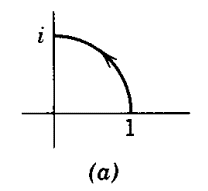
\includegraphics[width=\textwidth]{hw4-1}
	\end{subfigure}
	\begin{subfigure}[b]{0.1\textwidth}
		\centering
		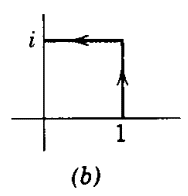
\includegraphics[width=\textwidth]{hw4-2}
	\end{subfigure}
\end{figure}

\textbf{Solution.}

Note that the function to be integrated is analytic, thus the integration result for all the paths are the same.
$$
I = \int_1^0 z \dd z + \int_0^i z \dd z = \frac{1}{2} - \frac{1}{2} = 0
$$

\newpage

\begin{Problem}
	
	Evaluate $\oint_C (\bar{z}-3) \dd z$ where $C$ is the indicated closed curve along the first quadrant part of the circle $|z| = 2$, and the indicated parts of the $x$ and $y$ axes. Hint: Don't try to use Cauchy's theorem!
	
\end{Problem}

\begin{figure}[h]
	\centering
	\begin{subfigure}[b]{0.1\textwidth}
		\centering
		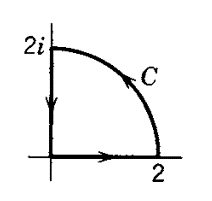
\includegraphics[width=\textwidth]{hw4-3}
	\end{subfigure}
\end{figure}

\textbf{Solution.}

$$
\begin{aligned}
	I &= \bigg(\int_0^2 + \int_{\text{Arc}} + \int_{2i}^0\bigg) (\bar{z}-3) \dd z\\
	&= 
\end{aligned}
$$




\newpage

\begin{Problem}
	
	Evaluate the following integrals:
	
	\noindent (a) $\oint_C \frac{\sin 2z \dd z}{6z-\pi}$ where $C$ is the circle $|z| = 3$
	
	\noindent (b) $\oint \frac{e^{3z} \dd z}{z - \ln 2}$ if $C$ is the square with vertices $\pm 1 \pm i$
	
\end{Problem}

\textbf{Solution.}

\newpage

\begin{Problem}
	
	For each of the following functions, say whether the indicated point is regular, an essential singularity, or a pole, and if a pole of what order it is.
	
	\noindent (a) $\frac{e^z-1-z}{z^2},\ z = 0$
	
	\noindent (b) $\frac{\sin z}{z^3},\ z = 0$
	
	\noindent (c) $\frac{z^2-1}{(z-1)^2},\ z = 1$
	
	\noindent (d) $\frac{\cos z}{(z-\pi/2)^4},\ z = \pi/2$
	
\end{Problem}

\textbf{Solution.}

\newpage

\begin{Problem}
	
	Find the residues of the following functions at the indicated points. Try to select the easiest of the methods outlined above. Check your results by computer.
	
	\noindent (a) $\frac{1}{(3z+2)(2-z)}$ at $z=-\frac{2}{3}$ and $z=2$
	
	\noindent (b) $\frac{z+2}{4z^2-1}$ at $z=\frac{1}{2}$ and $z=-\frac{1}{2}$
	
	\noindent (c) $\frac{\cosh z-1}{z^7}$ at $z=0$
	
	\noindent (d) $\frac{e^{iz}}{(z^2+4)^2}$ at $z=0$ and $z=\frac{1}{2}$
	
\end{Problem}

\textbf{Solution.}

\begin{comment}

\newpage

\begin{Problem}
	
	
	
\end{Problem}

\textbf{Solution.}

\newpage

\begin{Problem}
	
	
	
\end{Problem}

\textbf{Solution.}

\newpage

\begin{Problem}
	
	
	
\end{Problem}

\textbf{Solution.}

\newpage

\begin{Problem}
	
	
	
\end{Problem}

\textbf{Solution.}

\newpage

\begin{Problem}
	
	
	
\end{Problem}

\textbf{Solution.}

\newpage

\begin{Problem}
	
	
	
\end{Problem}

\textbf{Solution.}

\newpage

\begin{Problem}
	
	
	
\end{Problem}

\textbf{Solution.}

\end{comment}

\end{document}